\part{Production de graphiques}

\label{part:graphe}
\section{Introduction}
Il existe sous AIDA plusieurs outils de production de graphiques qui seront
décrits dans la suite de cette partie.

\begin{itemize}
    \item[•] \texttt{adp}             : visualisation des données d'une
                                        acquisition.
    \item[•] \texttt{vista}           : visualisation des données d'acquisitions
                                        sur toute une période.
    \item[•] \texttt{gengraphvect.py} : graphe de généalogie d'un vecteur.
    \item[•] \texttt{genparamvect.py} : graphe de généalogie d'un vecteur avec
                                        suivi d'un paramètre du header.
\end{itemize}

Ces outils peuvent être lancés en mode non-interactif ("\textit{mode batch}")
afin de produire des fichiers Quicklooks.
La génération automatique des fichiers Quicklook peut être faite
par la commande système \texttt{cron}.


\section{\texttt{adp} et son compagnon \texttt{adpbatch}}
\texttt{adp} (AIDA plot) permet de visualiser graphiquement les données d'une
acquisition.
Il permet également de créer un fichier de configuration qui pourra être
utilisé par son compagnon \texttt{adpbatch} pour générer des fichiers
Quicklooks en mode non-interactif ("\textit{mode batch}").

\subsection{Lancement}
\texttt{adp} peut être lancé sous \texttt{aito} par l'intermédiaire du bouton
\texttt{adp}
ou en ligne de commande dans un terminal. \\
Lancer la commande \fbox{ \texttt{adp -h} } pour obtenir de l'aide.

\subsection{Présentation}
La page principale de \texttt{adp} comporte plusieurs parties :

\begin{center}
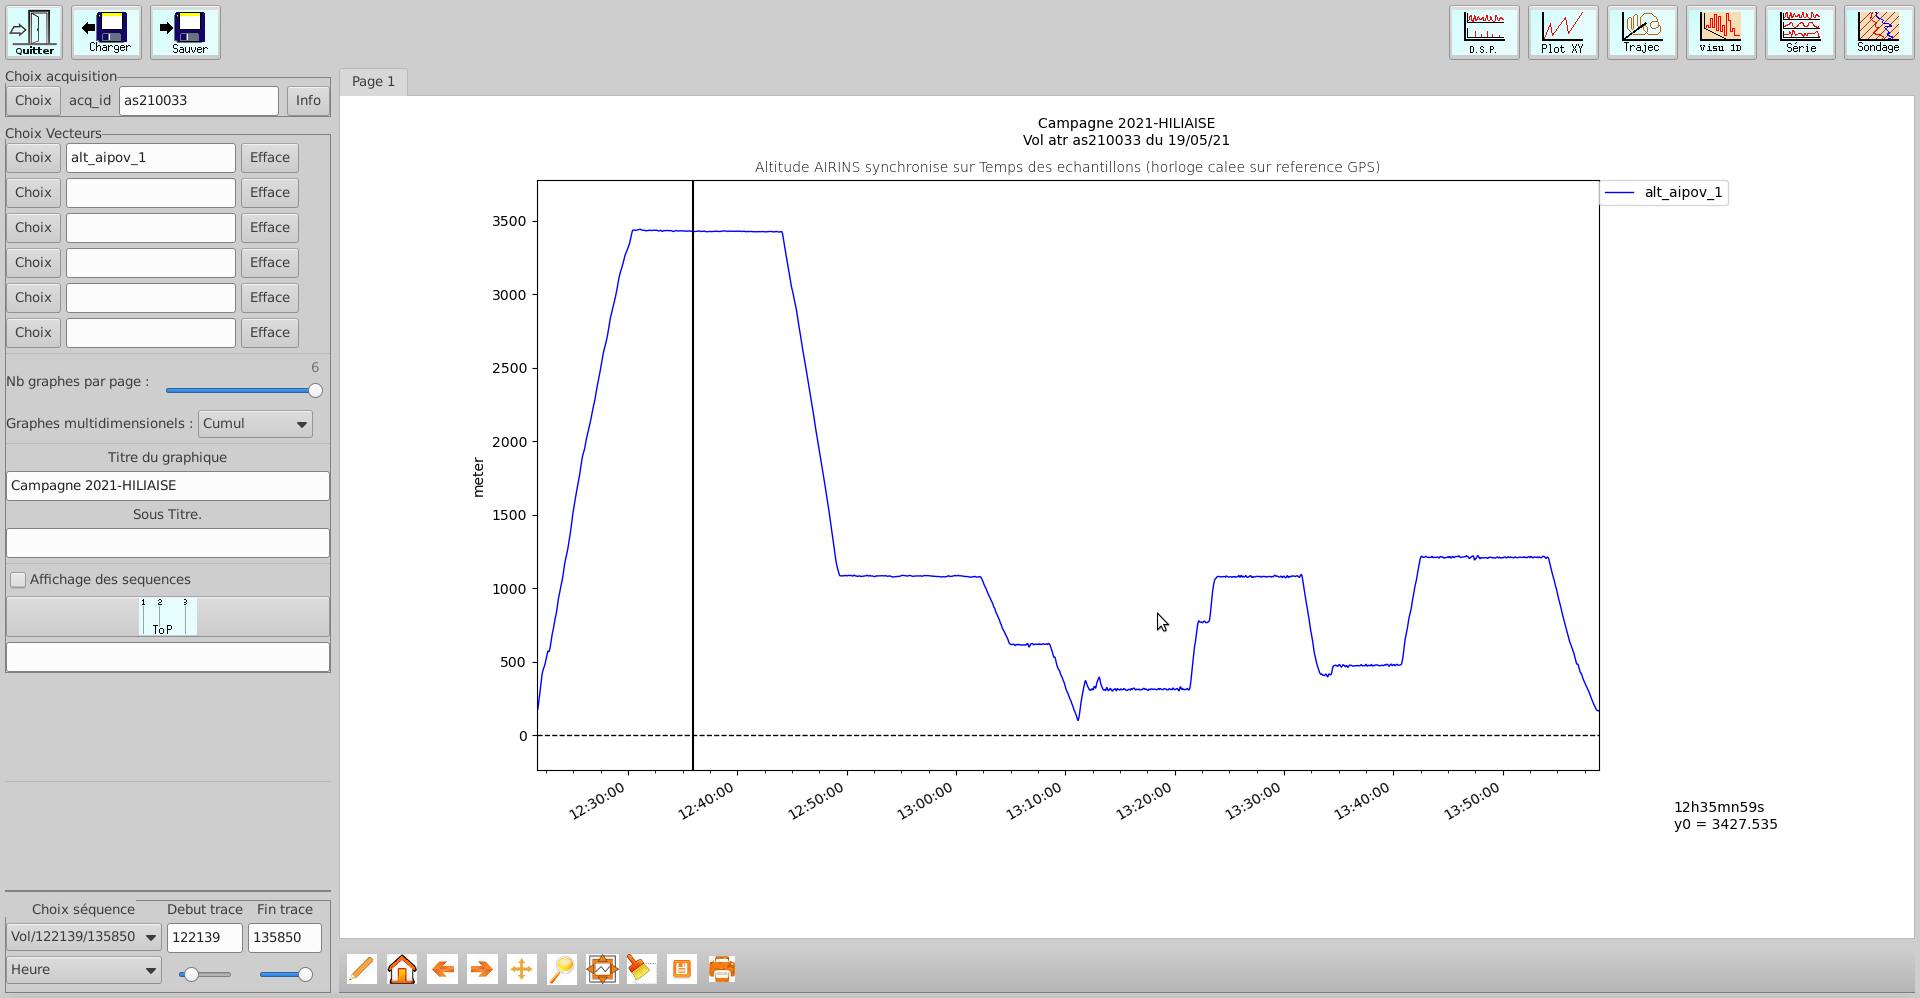
\includegraphics[width=14cm]{images/adp.png}
\end{center}

::: ICI : lorsque Pascal aura installé le manuel utilisateur, ajouter la ligne
Le \textbf{manuel de l'utilisateur} est accessible par le bouton \textbf{Aide}.


\section{\texttt{vista}}
\texttt{vista} (VIsualisation des Séries Temporelles AIDA) permet de
visualiser graphiquement les données d'acquisitions sur toute une période.
Il permet également de créer un fichier de configuration qui pourra être
utilisé pour générer des fichiers Quicklooks en mode non-interactif
("\textit{mode batch}").

\subsection{Lancement}
\texttt{vista} peut être lancé sous \texttt{aito} par l'intermédiaire du bouton
\texttt{vista}
ou en ligne de commande dans un terminal. \\
Lancer la commande \fbox{ \texttt{vista -h} } pour obtenir de l'aide.

\subsection{Présentation}
La page principale de \texttt{vista} comporte plusieurs parties :

\begin{center}
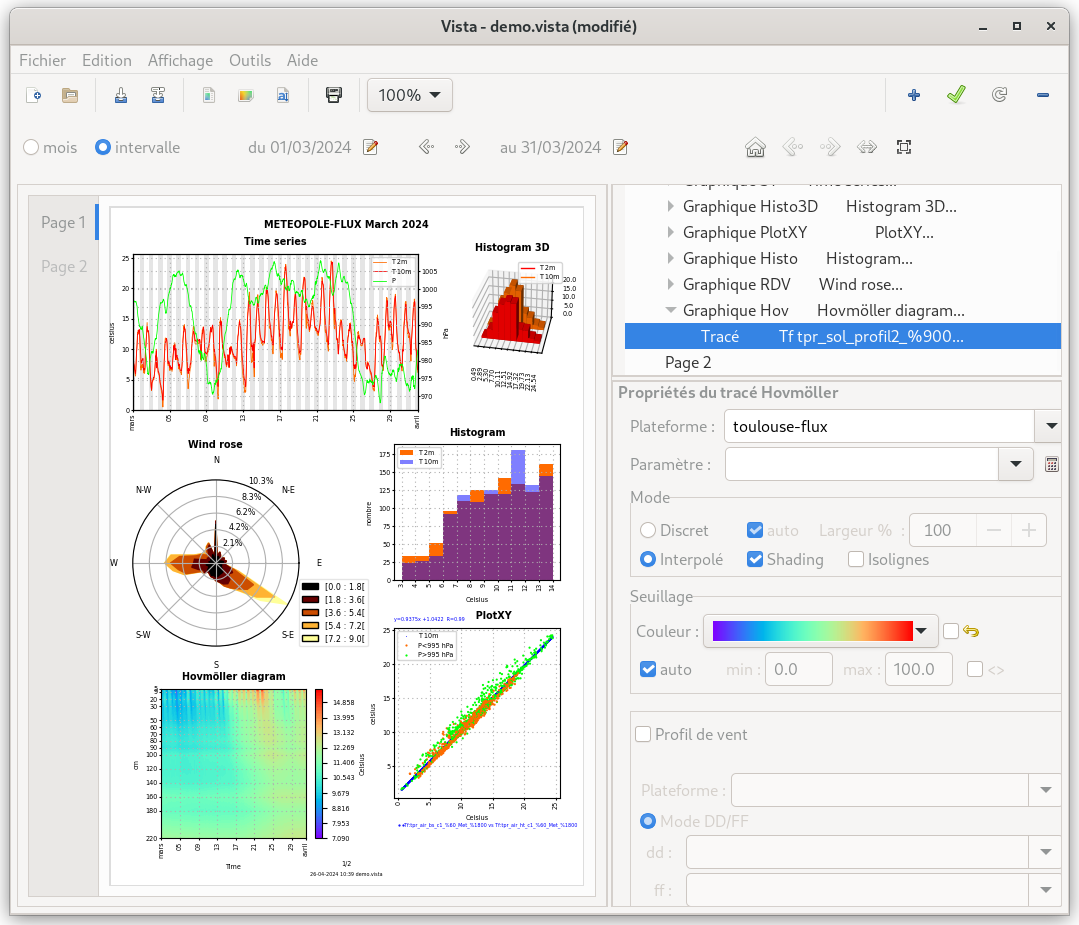
\includegraphics[width=14cm]{images/vista.png}
\end{center}

Le \textbf{manuel de l'utilisateur} est accessible sous l'entrée \textbf{Aide}
du menu principal.


\section{\texttt{gengraphvect.py}}
\texttt{gengraphvect.py} permet de générer le graphe généalogique d'un vecteur.

\subsection{Lancement}
\texttt{gengraphvect.py} peut être lancé sous \texttt{aito} (lorsqu'un vecteur
est sélectionné), par le bouton \texttt{arbre généalogique} de l'onglet
\texttt{données}
ou en ligne de commande dans un terminal. \\
Lancer la commande \fbox{ \texttt{gengraphvect.py -h} } pour obtenir de l'aide.

\medbreak
\textbf{\textit{Note : sous \texttt{aito}, \texttt{gengraphvect.py} est lancé
en mode \texttt{ascendant} avec l'opion de niveau : \texttt{3}}.}

\subsection{Présentation}
L'interface graphique de \texttt{gengraphvect.py} est déportée dans le
programme : \\
\texttt{\path{ihm_genere_graph_geneal_vect.py}} qui doit être lancé en ligne de
commande dans un terminal par la commande :
\fbox{ \texttt{\path{ihm_genere_graph_geneal_vect.py}} }.

\begin{center}
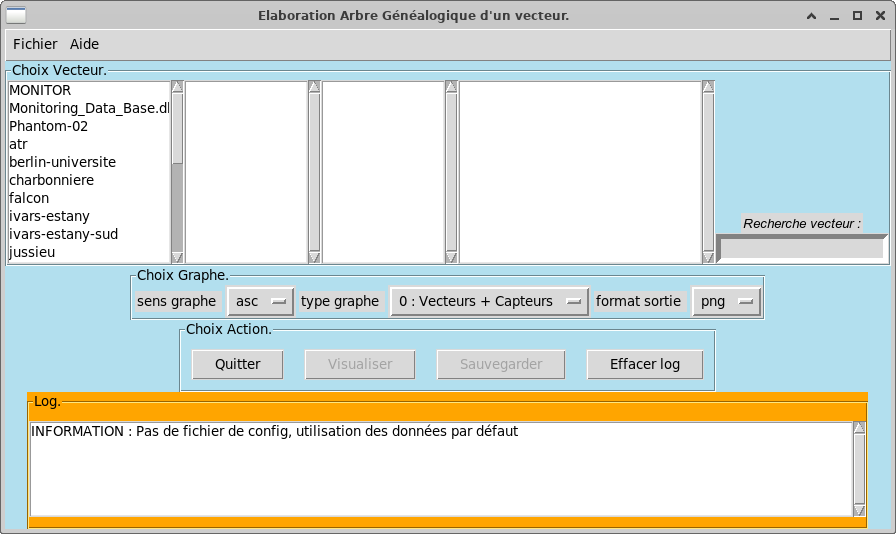
\includegraphics[width=14cm]{images/ihm_genere_graph_geneal_vect.png}
\end{center}

Le \textbf{manuel de l'utilisateur} est accessible sous l'entrée
\textbf{Aide/Doc Utilisateur} du menu principal.


\section{\texttt{genparamvect.py}}
\texttt{genparamvect.py} permet de générer le graphe généalogique d'un vecteur
en suivant un paramètre du header tel que l'unité.

\subsection{Lancement}
\texttt{genparamvect.py} doit ête lancé en ligne de commande un terminal. \\
Lancer la commande \fbox{ \texttt{genparamvect.py -h} } pour obtenir de l'aide.

